\chapter{Optimizing the Metric}
\label{sec:beta}

In a similar fashion as described in section \ref{chapter:alphalinkage} this sections aims to optimize a metric that is a linear combination of several metrics. For instance, images can have a 2D pixel representation and a text describing the each image. Combining these features for clustering tasks can be problematic as it is not how the optimal weight between these features should be. Does a word describe more than a subset of the image, are the features equally important or does the pixel image lead to better clusterings? With $\beta$-linkage we provide a framework based on $\alpha$-linkage that calculates different merges based on linear combinations of representations and leads to optimized clusterings.

\begin{figure}[h]
    \centering
    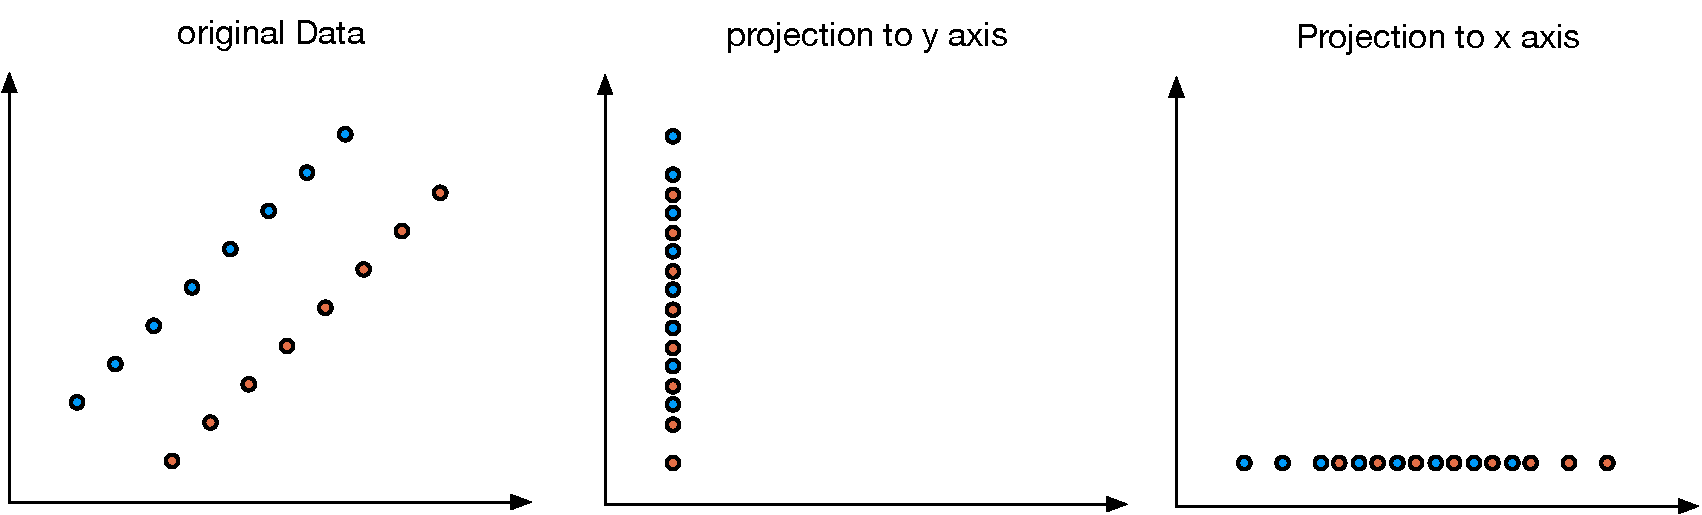
\includegraphics[width=0.7\textwidth]{images/ExampleDataset}
    \caption{Combining several metrics seems often natural and can lead to improved results as in this example where we project a dataset on both axes.}
    \label{fig:metrics}
\end{figure}

For instance, figure \ref{fig:metrics} shows a set of points that might be put in clusters easily. However, if you only look at the distance regarding the $X_1$-axis or the $X_2$-axis clustering will be very difficult, because each of the axis does not describe the spatial correlation anymore. This example is selected on purpose to motivate the following experiments where we learn optimal combinations of different metrics.

\todo[inline]{Explain difference to previous section.}